\section{Specifikationer}
FIR-filteret vælges til at være af type 1, altså er filterordenen $M$ lige og impulsresponsen $h[n]$ er symmetrisk, så $h[n] = h[M - n]$. Filteret har 2 knækfrekvenser $\omega_{c_1}$ og $\omega_{c_2}$ i rad/s, som vælges til at ligge midt imellem henholdsvis $\omega_1$ og $\omega_2$ samt $\omega_2$ og $\omega_3$. Derfor gælder der:
\begin{align*}
\omega_{c_1} &= \omega_1 + \dfrac{\omega_2 - \omega_1}{2} = \frac{\pi}{3} + \dfrac{\pi}{12} = \dfrac{5\pi}{12}, \\
\omega_{c_2} &= \omega_2 + \dfrac{\omega_3 - \omega_2}{2} = \frac{\pi}{2} + \dfrac{\pi}{8} = \dfrac{5\pi}{8}. \\
\end{align*}
Filtret designes dermed som et bånsstop filter med ovenstående knækfrekvenser. Den ideelle amplitude respons $H_d(\text{e}^{j\omega}$ er skitseret på figur \ref{fig:ideel_amp_respons} ud fra opstillede specifikationerne.   
\begin{figure}[H]
    \centering
    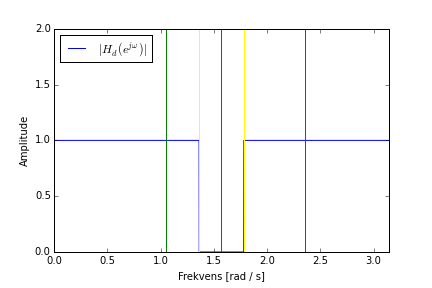
\includegraphics[width = 0.6\textwidth]{figures/ideel_amp_respons.PNG}
    \caption{Den ideelle amplituderespons for filteret.}
    \label{fig:ideel_amp_respons}
\end{figure}
